\documentclass[12]{article}
\usepackage[utf8]{inputenc}
\usepackage{float}
\usepackage[hidelinks]{hyperref}
\usepackage{graphicx}
\date{\today}
\author{Carlos Bergillos, Roger Vilaseca, Adrià Cabeza}
\title{Creación de dietas para ancianos: \\ sistemas Basados en el conocimiento \\
	\large IA FIB @ UPC}
\usepackage[margin=1.25in]{geometry}
\usepackage{listings}
\lstset{
	    basicstyle=\ttfamily,
	    showstringspaces=false,
	    commentstyle=\color{orange},
	    keywordstyle=\color{blue},
	    breaklines=true,numbers=none,
	    stringstyle=\color{red}, tabsize=3,   
	    showstringspaces=false,
	    columns=flexible,
	}
\begin{document}
\maketitle
\vspace*{\fill}
\begin{center}

\includegraphics[scale=0.5]{images/UPClogo.png}
\end{center}
\newpage
\tableofcontents
\newpage
\section{Introducción} 

Los \textbf{sistemas basados en el conocimiento (SBC)} son la parte de la Inteligencia Artificial donde se intenta hallar una solución utilizando el conocimiento. Hay ciertos problemas en la vida real que no se pueden resolver sin tener conocimiento específico sobre los elementos del dominio. 
\par
El motivo de esta práctica es comprender estos modelos de IA. Por eso hemos atacado un problema con esta técnica. El problema en cuestión ha sido la creación de menús para ancianos dependiendo de sus necesidades nutricionales y requisitos médicos. 
\par
Hemos desarrollado una ontología capaz de almacenar la información sobre los platos, los ingredientes, los nutrientes, las enfermedades y las limitaciones con \textbf{Protégé} y un sistema de reglas que describen el proceso de toma de decisiones usando \textbf{CLIPS}.
\par
Para atacar el problema de una manera adecuada hemos utilizado las diferentes fases de la metodología de ingeniería del conocimiento: 

\begin{itemize}
	\item \textbf{Identificación}, donde identificaremos el problema y sus características y requisitos. Además también concretaremos el dominio para poder identificar las fuentes de conocimiento necesarias para su desarrollo.%DONE
	\item \textbf{Conceptualización}, donde describiremos en profundidad los conceptos que intervienen en el dominio del problema y la descomposición de este último en subproblemas. %ALMOST DONE, FA FALTA AFEGIR INFO SOBRE ELS CONCEPTES QUE TENIM AL DOMINI
	\item \textbf{Formalización}, donde partiendo de los conceptos de la fase anterior, procediremos a su formalización desarrollando una ontología. También, para la resolución del problema formalizaremos el conocimiento y una metodología de resolución.
\item \textbf{Implementación}, donde dividiremos el problema en módulos para encapsular las diferentes partes del procedimiento en la resolución descrita en la fase anterior. Esta fase se basará en una metodología de desarrollo incremental, partiendo de un prototipo inicial que se va aumentando hasta conseguir un sistema final. 
\item \textbf{Prueba}, donde mediante juegos de prueba testearemos diferentes aspectos, en especial los más críticos, del sistema. 
\end{itemize}

\section{Identificación}
En este primer apartado del trabajo, describiremos el problema, sus distintas partes y las fuentes de información que requieren. Además añadiremos un análisis de viabilidad acerca la opción de utilizar un SBC para su resolución.

\subsection{Descripción del problema}
La alimentación es una pieza clave de nuestras vidas: nuestra manera de alimentarnos define nuestra salud, tanto física como mental. Con nuestra alimentación podemos prevenir el riesgo y agravamiento de enfermedades y mantener un nivel óptimo de salud. Para obtener una \textbf{buena alimentación} necesitamos consumir una cantidad equilibrada de nutrientes, integrada por nutrientes, vitaminas, proteínas, lípidos...
\\
Además cuando nos hacemos mayores nuestra salud se vuelve más frágil y quebradiza. Debido a eso, cuantos más años tenemos, más tenemos que vigilar nuestra alimentación.
\\
En esta práctica desarrollaremos una solución para este problema. Una solución basada en un sistema basado en el conocimiento que sea capaz de generar menús semanales personalizados adecuados a las características de una persona según su edad, sus restricciones de dieta considerando sus enfermedades y sus preferencias generales sobre la comida.\\

Por ejemplo, si una persona es vegetariana y además diabética, se le generaría un menú sin carne y con poca cantidad de azúcares. Además tal y como hemos mencionado, nuestro sistema también admite preferencias, así pues a una persona que tenga osteroporosis y no le guste nada la verdura se le intentará asignar un menú que contenga calcio y que no tenga platos con verduras. 

\subsection{Viabilidad de utilizar un SBC}
Si analizamos el problema, podemos observar que no es un problema que se pueda resolver simplemente con algoritmos, sinó que el sistema requiere, para poder operar, de un conocimiento de nutrición salud.
\\
Además nuestro objetivo, como ya hemos mencionado anteriormente, es dada la información de un anciano como input es dar una solución viable. Así que un SBC parece una opción bastante apropiada para enfretarse al problema. 
\medskip

Pese a que se podría utilizar otros métodos como la satisfacción de restricciones o incluso mediante una búsqueda en el espacio de soluciones creemos que la mejor manera de aprovechar el conocimiento implícito que requiere el problema es usando la potencia que nos proporciona un sistema basado en conocmiento.

\subsection{Fuentes de conocimiento}

Nuestras fuentes de conocimiento se pueden dividir en dos grandes pilares:
\begin{itemize}
	\item \textbf{El usuario}: la persona que utilize nuestro sistema tendrá que indicar e introducir información acerca de su edad, sexo, enfermedades...para que podamos proporcionarle el mejor plan alimenticio. 
	\item \textbf{Platos, ingredientes, enfermedades, nutrientes, etc}: el conjunto de conocimiento que necesita nuestro SBC para poder operar ha sido obtenido utilizando recursos en la red, especialmente se ha usado documentación especializada en el tema. 
\end{itemize}


\subsection{Objetivos y resultados esperados del sistema}
El objetivo final del problema es mostrar un menú para toda la semana que sea adecuado a las necesidades alimentícias del usuario. 
\medskip

Para esto el sistema tiene que cumplir una serie de objetivos: 
\begin{itemize}
	\item Obtener todos los datos del usuario que sean necesarios para poder utilizar el conocimiento del sistema y así poder devolver el mejor resultado posible
	\item Inferir sobre las características del usuario de forma que obtengamos un conjunto de platos específicos para el usuario
	\item Presentar al usuario el menú semanal (7 días) obtenido por el sistema		
\end{itemize}

Así pues esperamos de nuesto sistema un comportamiento que cumpla todos los objetivos indicados arriba para finalmente obtener unos resultados aceptables que esten concorde con el conocimiento del sistema. 
\section{Conceptualización}
En este apartado describiremos todos los conceptos del dominio. 

\subsection{Conceptos del dominio}
\begin{itemize}
\item \textbf{Persona}: las características necesarias para definir correctamente a la persona (usuario) son: \begin{itemize}
	\item \textbf{Edad}: tiene que ser $>=$ 65 ya que el sistema está orientado a ancianos
	\item \textbf{Género}: ya que dependiendo del sexo se tienen que seguir unas restricciones alimentícias u otras.
	\item \textbf{Nivel de ejercicio semanal}: que puede ser Sedentario, Activo o Vigorosamente Activo
	\item \textbf{Enfermedades que padece}
	\item \textbf{Preferencias alimenticias}: que pueden ser Vegetariano, Vegano o Musulmán
	\end{itemize}
	
	\item \textbf{Platos}
	\begin{itemize}
		\item \textbf{Temporadas}: pueden ser Otoño, Verano, Invierno y/o Primavera
		\item \textbf{Ingredientes}		
	\end{itemize}

	\item \textbf{Ingredientes}: las caracerístias necesarias para definir correctamente a un ingrediente son las siguientes: \begin{itemize}
		\item \textbf{Nutrientes} Los nutrientes que contiene el ingrediente en cuestión
		\item \textbf{Nombre}
		\item \textbf{Temporadas}: pueden ser Otoño, Verano, Invierno y/o Primavera
		\item \textbf{Tipo}: \begin{itemize}
			\item \textbf{Dairy and Egg Products}: donde se incluyen leche o huevos y sus derivados.
			\item \textbf{Spices and Herbs}: donde se incluyen especias y hierbas .
			\item \textbf{Fats and Oils}: donde se incluyen grasas y aceites varios.
			\item \textbf{Poultry Products}: donde se incluyen aves de todo tipo: gallinas, pavos, patos,etc.
			\item \textbf{Fruits and Fruit Juices}: donde se incluyen frutas y zumos varios. 
			\item \textbf{Pork Products}: donde se incluyen los productos que contienen cerdo.
			\item \textbf{Vegetables and Vegetable Products}: donde se incluyen verduras y vegetales.
			\item \textbf{Nut and Seed Products}: donde se incluyen semillas y frutos secos.
			\item \textbf{Beef Products}: donde se incluyen carnes de vacuno.
			\item \textbf{Sausages and Luncheon Meats}: donde se incluyen salchichas y embutidos.
			\item \textbf{Finfish and Shellfish Products}: donde se incluyen pescados y marisco.
			\item \textbf{Legumes and Legume Products}: donde se incluyen legumbres y derivados.
			\item \textbf{Sweets}: donde se incluyen dulces.
			\item \textbf{Soups, Sauces, and Gravies}: donde se incluyen sopas, salsas.
			\item \textbf{Snacks}: donde se incluyen aperitivos varios.
			\item \textbf{Breakfast Cereals}: donde se incluyen cereales.
			\item \textbf{Baked Products}: donde se incluyen productos horneados.
			\item \textbf{Lamb, Veal, and Game Products}: donde se cordero y productos de caza.
			\item \textbf{Cereal Grains and Pasta}: donde se incluyen granos de cereales y tipos de pasta.
			\end{itemize}
		\end{itemize}
	\item \textbf{Nutrientes}: formado por los valores nutricionales que hemos considerado más importantes y adecuados para realizar nuestro sistema. Entre ellos se encuentran: 
	\begin{itemize} 
		\item Grasa
		\item Carbohidratos
		\item Calorías
		\item Sucrosa
		\item Glucosa
		\item Fructosa
		\item Lactosa
		\item Cafeína
		\item Alcohol
		\item Azúcar
		\item Colesterol
		\item Grasas de las cuáles saturadas
		\item Calcium
	\end{itemize}


\item \textbf{Enfermedades}: cada enfermedad, además de su nombre la cual nos sirve para definirla en sí, tenemos para cada enfermedad el conocimiento de qué limitaciones alimentícias presentan. \begin{itemize}
	\item \textbf{Nombre}
	\item \textbf{Limitaciones}: pueden ser limitaciones asociadas a nutrientes o a ingredientes.
	\item Nuestro SBC admite actualmente las siguientes enfermedades:
		\begin{itemize}
		\item Diabetes
		\item Celiaquía
		\item Colesterol
		\item Gota
		\item Hipertension
		\item Cirrhosis
		\item Anemia
		\item Osteoporosis / Arthritis
		\end{itemize}
\end{itemize}
\end{itemize}


\subsection{Problemas y subproblemas}

Uno de los mejores métodos para trabajar con grandes problemas como este es dividirlos en varios subproblemas más pequeños para poderlo solucionar.

En nuestro caso lo vamos a dividir entre los siguientes 4:

\subsubsection{Recogida de información personal}

En esta parte del problema realizaremos varias preguntas al usuario, donde obtendremos la suficiente información para luego poder ser usado y obtener un menú adecuado a las condiciones y gustos de la persona.

\subsubsection{Análisis de los datos personales}

Una vez obtenidos los datos de la persona, el experto clasificará mediante una puntuación los diferentes platos según lo adecuados que sean para la persona. Para esto tendremos en cuenta si la persona tiene alguna enfermeda, alguna preferencia alimentaria, su religión o que clase de alimentos prefiere.

\subsubsection{Filtrado de platos para el menú}

Para decidir que platos entran en el menú primero de todo vamos a coger los 7 desayunos y los 15 postres mejor puntuados del apartado anterior y los vamos a fijar en nuestro menú. A continuación fijaremos todos los primeros platos menos 4 y todos los segundos platos menos 5 (cogiendo los que tengan mejor puntación).
Finalmente con los platos que falten, haremos diferentes permutaciones para encontrar los platos que sean mas adecuado para la cantidad de calorias necesarias para la persona.

\subsubsection{Impresión del menú}

Una vez tengamos el menú construido vamos a sacar por pantalla el menú final de la semana, donde por cada plato habrá sus ingredientes.
Después del menú va a salir la información nutricional del menú obtenido, comparados con los resultados que deberíamos tener a partir de la información que nos ha dado la persona en el primer subproblema.

\subsection{Ejemplos del conocimiento extraído del dominio}
%aquí deberíamos explicar como hemos ido desarrollando prototipos de la implementación para demostrar que hemos usado una metodología incremental 
A partir de información que obtenemos del dominio podemos llegar a clasificar los platos en función de las características y peticiones de cada persona.

Por ejemplo a partir de las siguientes características o preferencias que podríamos obtener a partir de las preguntas hechas, obtendríamos los siguientes resultados.

\begin{itemize}
	\item En el caso de los vegetarianos vamos a quitar de los posibles platos aquellos que tengan algún ingrediente del tipos carne.
	\item Si la persona tuviera diabetes vamos a intentar que los platos sugeridos tengan poca cantidades de azúcares.
	\item En cambio si la persona responde que le gusta un alimento en concreto vamos a puntuar de una forma más alta aquellos platos que contengan el alimento en cuestión.
\end{itemize}

\subsection{Flujo de razonamiento}

Para poder clasificar correctamente los platos en nuestro problema a partir de las preguntas hechas.

Primero de todo pasaremos un filtro donde se eliminaran del conjunto de platos, aquellos que la persona no puede tomar en ninguna circunstancia.

A continuación los platos que hayan pasado de la opción anterior serán puntuados para prioriza que platos debe o no debe tomar dicha persona.

Al final obtendremos una lista ordenada de los mejores platos para la persona, con los cuales diseñaremos el menú más adecuado para cada usuario. 


\section{Formalización}

\subsection{Desarrollo de la ontología}
Para desarrollar correctamente la ontología hemos procurado que todos los conceptos del dominio sean representables. En este caso, los términos más importantes de la ontología son los \textbf{platos}, puesto que nuestra solución será un conjunto de ellos, los \textbf{ingredientes} y sus \textbf{características nutricionales} y los conceptos relacionados con el usuario: \textbf{preferencias} y \textbf{enfermedades}. Además para poder representar bien los susodichos conceptos, hemos creído conveniente hacer uso de clases auxiliares para definir cantidades. Así pues, por ejemplo para definir que un plato contiene una cantidad de un ingrediente en concreto usaríamos la clase \textit{IngredientQuantity}.
\label{ontologia_apartado}
\subsubsection{Definición de clases y jerarquía}

La ontología que hemos realizado para nuestro SBC contiene diversas clases. Se puedens observar en la \autoref{fig_ontologia}.

\begin{figure}[H]
\centering
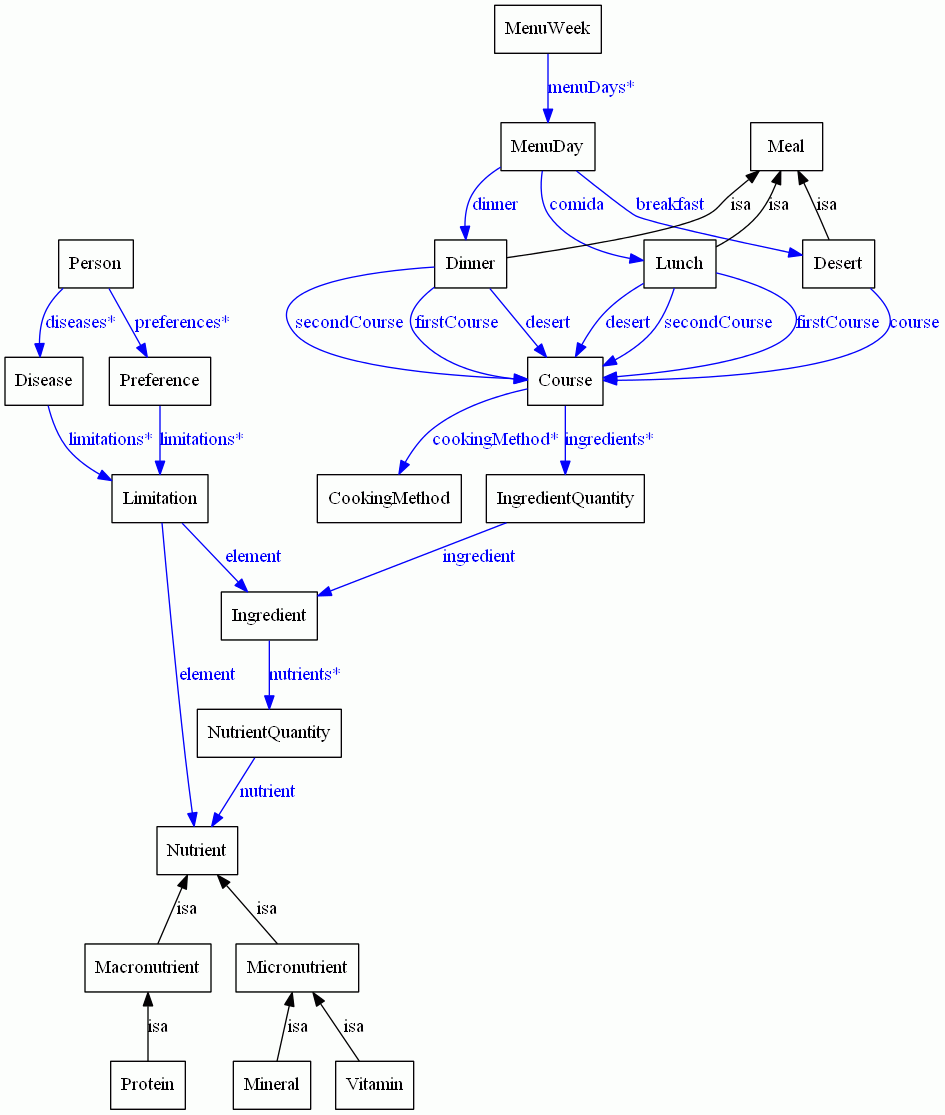
\includegraphics[width=\textwidth,height=\textheight,keepaspectratio]{images/full_light.png}
\caption{Ontología completa de nuestro SBC}
\label{fig_ontologia}
\end{figure}

\vspace{0.5cm}

A continuación detallaremos cada una de las clases.

\paragraph{Clase \emph{Course}}\mbox{}\\
\begin{figure}[H]
\centering
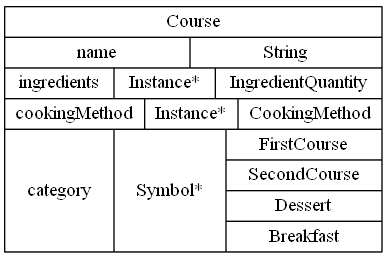
\includegraphics[scale=0.5]{images/class_Course.png}
\caption{Clase \emph{Course}}
\label{fig_class_Course}
\end{figure}

Definimos aquí toda la información que contiene un plato. Tenemos, entre otras cosas, la información acerca de los ingredientes que contiene y sus cantidades además de la categoría a la que pertenece que puede ser primer plato, segundo plato, postre o desayuno.
\\

Los atributos son:
\begin{itemize}
\item \textbf{name}: nombre del plato
\item \textbf{ingredients}: lista de ingredientes que contiene el plato, y sus cantidades
\item \textbf{cookingMethod}: método que se utiliza para cocinar el plato; i.e. hervir, freír...
\item \textbf{category}: categoría del plato; puede ser primer plato, segundo plato, desayuno o postre. 
\end{itemize}


\vspace{0.5cm}

\paragraph{Clase \emph{Ingredient}}\mbox{}\\
\begin{figure}[H]
\centering
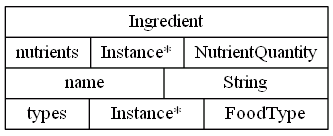
\includegraphics[scale=0.5]{images/class_Ingredient.png}
\caption{Clase \emph{Ingredient}}
\label{fig_class_Ingredient}
\end{figure}

Definimos aquí toda la información que contiene un ingrediente. Por ejemplo, los valores nutricionales que presenta el ingrediente.
\\

Los atributos son: 
\begin{itemize}
\item \textbf{name}: nombre del ingrediente
\item \textbf{nutrients}: lista de nutrientes del ingrediente, y sus cantidades
\end{itemize}


\vspace{0.5cm}


\paragraph{Clase \emph{IngredientQuantity}}\mbox{}\\
\begin{figure}[H]
\centering
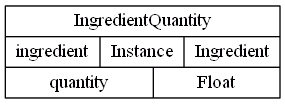
\includegraphics[scale=0.5]{images/class_IngredientQuantity.png}
\caption{Clase \emph{IngredientQuantity}}
\label{fig_class_IngredientQuantity}
\end{figure}

Para poder expresar la cantidad de ingredientes que contiene un plato hacemos uso de esta clase la cual contiene una referencia a una instancia ingrediente y la cantidad que hay en ese plato del ingrediente.
\\

Los atributos son:
\begin{itemize}
\item \textbf{ingredient}: ingrediente
\item \textbf{quantity}: cantidad del ingrediente
\end{itemize}


\vspace{0.5cm}

\paragraph{Clase \emph{Nutrient}}\mbox{}\\
\begin{figure}[H]
\centering
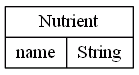
\includegraphics[scale=0.5]{images/class_Nutrient.png}
\caption{Clase \emph{Nutrient}}
\label{fig_class_Nutrient}
\end{figure}

Definimos en esta clase toda la información que contiene un nutriente.
Aunque la clase actualmente solo contiente un atributo para el nombre, representa un concepto lo suficientemente importante en nuestra ontología como para merecer su propia clase, ya que en futuros proyectos esta clase podria requerir otros atributos.
\\

Los atributos son:
\begin{itemize} 
\item \textbf{name}: nombre del nutriente
\end{itemize}

\vspace{0.5cm}

\paragraph{Clase \emph{NutrientQuantity}}\mbox{}\\
\begin{figure}[H]
\centering
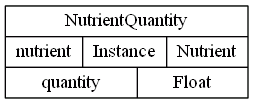
\includegraphics[scale=0.5]{images/class_NutrientQuantity.png}
\caption{Clase \emph{NutrientQuantity}}
\label{fig_class_NutrientQuantity}
\end{figure}

Para poder expresar la cantidad de nutrientes que contiene un ingrediente en concreto hacemos uso de esta clase. Esta dispone de una referencia a una instancia de nutriente además de la cantidad que ese nutriente en ese ingrediente (las unidades han sido normalizadas en gramos). 
\\

Los atributos son: 
\begin{itemize}
\item \textbf{nutrient}: nutriente
\item \textbf{quantity}: cantidad del nutriente
\end{itemize}


\vspace{0.5cm}

\paragraph{Clase \emph{Disease}}\mbox{}\\
\begin{figure}[H]
\centering
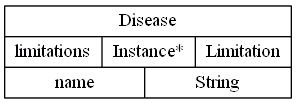
\includegraphics[scale=0.5]{images/class_Disease.png}
\caption{Clase \emph{Disease}}
\label{fig_class_Disease}
\end{figure}

Definimos en esta clase toda la información que contiene una enfermedad. En nuestro caso, una enfermedad presenta una serie de limitaciones alimentícias.
\\

Los atributos son: 
\begin{itemize}
\item \textbf{limitations}: limitaciones alimentícias que suponen la enfermedad
\item \textbf{name}: nombre de la enfermedad
\end{itemize}

\vspace{0.5cm}

\paragraph{Clase \emph{Preference}}\mbox{}\\
\begin{figure}[H]
\centering
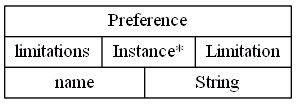
\includegraphics[scale=0.5]{images/class_Preference.png}
\caption{Clase \emph{Preference}}
\label{fig_class_Preference}
\end{figure}

Definimos en esta clase toda la información que contiene una preferencia. En la práctica, una instancia de esta clase se comporta de forma muy parecida a la de una de la clase \emph{Disease}. Pero aunque las preferencias tengan tambien una lista de limitaciones, estas suelen ser menos estrictas que las de una enfermedad, e incluso puede tratarse de preferencias positivas, en las que se quiere propiciar el uso de ciertos alimentos o nutrientes.
\\

Los atributos son: 
\begin{itemize}
\item \textbf{limitations}: limitaciones positivas o negativas asociadas a la preferencia
\item \textbf{name}: nombre de la preferencia
\end{itemize}

\vspace{0.5cm}

\paragraph{Clase \emph{Limitation}}\mbox{}\\
\begin{figure}[H]
\centering
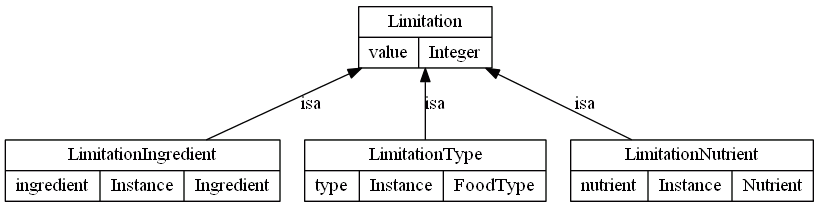
\includegraphics[scale=0.5]{images/class_Limitation.png}
\caption{Clase \emph{Limitation}}
\label{fig_class_Limitation}
\end{figure}

Para ser capaces de expresar una limitación o incluso una preferencia alimentícia, hemos hecho uso de esta clase para poder describir la voluntad de castigar o premiar el uso de ciertos alimentos o nutrientes.
\\

Existen tres tipos (subclases) de la clase \emph{Limitation} según el objetivo de la limitación:
\begin{itemize}
\item \emph{\textbf{LimitationIngredient}}: dirigido a influir en el uso de un ingrediente asociado
\item \emph{\textbf{LimitationType}}: dirigido a influir en el uso de un tipo de ingrediente asociado (i.e. carne)
\item \emph{\textbf{LimitationNutrient}}: dirigido a influir en el uso de los ingredientes que contengan el nutriente asociado

\end{itemize}

A parte de la instancia asociada según la subclase, las limitaciones también disponen del siguiente atributo:
\begin{itemize}
\item \textbf{value}: valor númerico asociado a la limitacion. Se usan valores negativos para castigar el uso de ingredientes y nutrientes, y valores positivos para premiarlo. La magnitud del valor indica la severidad con la que se quiere hacer efectiva la limitación. Un valor de 0 indica una limitación neutral y no tiene ningún efecto. 
\end{itemize}




\subsection{Método de resolución}

En los problemas de SBC, donde se debe a partir de una preguntas obtener una solución adecuada, se realiza mediante una clasificación heurística.
Los problemas que se resuelven mediante clasificación heurística se pueden dividir en tres partes:

\subsubsection{Abstracción de los datos}

En esta parte del problema pasaremos de un problema concreto a un problema abstracto. 
Obteniendo los datos de la persona (condiciones físicas, enfermedades, preferencias alimentarias...), el sistema abstraerá los datos necesarios por tal de poder ser usados luego para encontrar la mejor situación.
En nuestro caso podemos encontrar esta parte del problema en los módulos MAIN, ask\_questions.

\subsubsection{Asociación heurística}

En esta parte pasaremos del problema abstracto a una solución abstracta.
A partir de los diferentes datos del problema abstracto obtenido en la primera parte, obtendremos una solución abstracta, la cual consistirá en puntuar los diferentes platos según lo convenvenientes que sean para la persona.
Por ejemplo una persona vegetariana obtendrá una puntuación menor para los platos que contengan carne.
También en esta parte haremos el cálculo de Harris Benedict para obtener el número de calorías que necesita una persona al día.
De esta forma tendremos una lista ordenada de los platos mas recomendados para cada usuario.
Esta parte lo podemos encontrar en el modulo inference\_of\_data.

\subsubsection{Adaptación}

Finalmente la Adaptación consiste en pasar de la solución abstracta a la solución concreta.
Aquí cogeremos las listas de platos ordenadas i repartiremos estos platos en un menú dónde cada día se cumpla el número de calorías necesarias.
Finalmente sacaremos por pantalla el menú obtenido para la persona i la cantidad de calorías que contiene.
La adaptación esta formada por los módulos generate\_solutions i printing.

\section{Implementación}

\subsection{Creación de la ontología}
Para generar la ontología hemos usado el programa Protégé añadiendo varias características y atributos para poder representar nuestros conceptos del dominio y crear nuestras soluciones.
\\
En cuanto a las instancias, hay una distinción básica entre ellas: estáticas y dinámicas. Hay algunas que se han creado dinámicamente durante la ejecución del programa como podrían ser Persona o MenúDía. Para las estáticas en cambio (Nutriente, Plato, Ingrediente, IngredienteCantidad, NutrienteCantidad, Enfermedad o Limitaciones) hemos usado diversas bases de datos y un script en python para crearlas a priori y tener los archivos .pins necesarios. 
\subsection{Módulos}
Con el intento de facilitar la resolución del problema y la lectura del código, este ha sido dividido de diferentes módulos que se van activando por conveniencia.
\par
Dichos módulos son los siguientes:
\begin{itemize}
	\item \textbf{Módulo MAIN}: es el módulo principal del sistema. Contiene una serie de funciones útiles para los otros módulos y la regla que inicia la ejecución del sistema. 
	\item \textbf{Módulo ask\_questions}: este módulo recopila toda la información que se necesita del usuario. Esta información se recopila mediante una serie de preguntas. 
	\item \textbf{Módulo inference\_of\_data}:este módulo realiza todo el procesado de la información aportada por el ususario para poder generar la solución. En este módulo se calculan las calorías que necesita el usuario y se les asigna la puntuación a los platos dependiendo de sus preferencias, enfermedades.  
	\item \textbf{Módulo generate\_solutions}: este módulo contiene las reglas que generan nuestro menú semanal.
	\item \textbf{Módulo printing}: la función de este módulo es printar la información al usuario y finalizar la ejecucción
\end{itemize}



\subsection{Prototipos}
Tal y como se ha mencionado anteriormente, hemos seguido para el desarrollo de la práctica un método incremental por prototipos. Este tipo de desarrollo nos ha permitido avanzar de manera más organizada y paulatina. 
\\
En un inicio, desarrollemos nuestro \textbf{prototipo inicial}: una ontología bastante completa (muy parecida a la que se ha utilizado en la versión final) y un sistema que hacía preguntas y creaba un menú totalmente random.  Nos sirvió para empezar a familiarizarnos con \textbf{Protégé} y \textbf{CLIPS} y en cómo tenían que ser las instancias. Después iteremos sobre ese prototipo: creemos un script en \textbf{Python} para facilitarnos la creación de las instancias y empezemos a añadir las primeras reglas básicas (i.e. restricciones de vegetariano). 
\\
Entonces después de hacer unos pequeños cambios en la ontología y por consiguiente en el script para crear instancias, procedimos a crear, de manera progresiva, las diferentes reglas inherentes al conocimiento: enfermedades, limitaciones, preferencias, etc.

\section{Juego de Prueba}
Una vez implementado nuestro SBC, hemos realizado una serie de pruebas enfocadas a testear diferentes puntos de la aplicación. Así pues, mediante estas pruebas, hemos podido comprovar el correcto funcionamento del sistema, tanto a nivel general como a nivel particular.

\subsection{Prueba 1: Usuario Estándard}
\subsubsection{Descripción del caso}
En nuestro primer caso de prueba hemos querido probar el buen funcionamiento de nuestro SBC con casos estándard. 
\medskip

Nuestro test incluye:
Un \textbf{hombre genérico}, sin preferencias alimenticias y que no padece ninguna enfermedad.

\begin{itemize}
\item \textbf{Sexo}: Hombre
\item \textbf{Edad}: 80
\item \textbf{Peso}: 65kg
\item \textbf{Altura}: 170cm
\item \textbf{Actividad Física}: Sedentario
\end{itemize}

\subsubsection{Solución esperada}
Esperamos obtener una solución que esté acorde con las necesidades calóricas del individuo, los cuales dependen de la altura, el sexo, la actividad física y el peso.

\subsubsection{Resultado obtenido}

\subsection{Prueba 2: Mujer diabética con preferencias alimentícias}
En este caso hemos querido probar como funcionaba nuestro SCB con una \textbf{mujer diabética con ciertas preferencias alimentícias}. La mujer en cuestión \textbf{prefiere comer verduras y sopas y no prefiere alimentos con grasas y/o aceites}.  

\begin{itemize}
\item \textbf{Sexo}: Mujer
\item \textbf{Edad}: 85
\item \textbf{Peso}: 60kg
\item \textbf{Altura}: 160cm
\item \textbf{Actividad Física}: Sedentaria
\end{itemize}

\subsubsection{Solución esperada}
Esperamos obtener una solución que esté acorde con las necesidades calóricas del individuo. Además también esperamos obtener un menú con platos con cantidades bajas de azúcar; una presencia baja o nula de aceites o grasa y una disposición de platos que sean sopas o tengan verduras.

\subsubsection{Resultado obtenido}

\subsection{Prueba 3: Hombre Musulmán que necesita muchas calorías}
En este caso hemos querido probar como se comporta nuestro SBC cuando se requiere \textbf{una gran cantidad de calorías}. Además para restringir más el espacio de soluciones, hemos insertado la restricción de ser \textbf{musulmán}, hecho que hace que se intente \textbf{eliminar la presencia de alimentos con cerdo}. 

\begin{itemize}
\item \textbf{Sexo}: Hombre
\item \textbf{Edad}: 80
\item \textbf{Peso}: 60kg
\item \textbf{Altura}: 170cm
\item \textbf{Actividad Física}: Muy activo
\end{itemize}

\subsubsection{Solución esperada}
Tal y como hemos mencionado anteriormente, este caso está creado primeramente para testear el comportamiento del SCB con un requerimiento de muchas calorías, así que no sería extraño que obtuviéramos un menú que no se adecua a esos requisitos. También deberíamos obtener un menú con poco/nada cantidad de cerdo en sus platos. 
\\
Además, puesto que el requisito de la carne de cerdo tiene más peso que el de las calorías, esperemos poder ver un output que lo refleje. 

\subsubsection{Resultado obtenido}

Como resultado hemos obtenido un menú con menos calorías de las que deberían, 

\subsection{Prueba 4: Mujer con gota que necesita pocas calorías con preferencias alimentícias}

En este caso hemos querido probar como funcionaba nuestro SBC con una \textbf{mujer con gota y que necesita pocas calorías}. La mujer en cuestión además tiene \textbf{preferencias alimentícias que no están acorde con la enfermedad}. Es decir, prefiere comer carne y marisco cuando su enfermedad se lo restringe. 

\begin{itemize}
\item \textbf{Sexo}: Mujer
\item \textbf{Edad}: 92
\item \textbf{Peso}: 72kg 
\item \textbf{Altura}: 168cm
\item \textbf{Actividad Física}: Sedentaria
\end{itemize}

\subsubsection{Solución esperada}
Esperamos obtener una solución que esté acorde con los requisitos alimentícios de la gota. Es importante mencionar que las preferencias de la persona son contrarias a las restricciones de la enfermedad. No obstante, debido a que las restricciones de enfermedad tienen más peso que las otras, esperamos seguir obteniendo un buen resultado. Además también queremos probar como se comporta nuestro sistema cuando el individuo necesita una cantidad muy pequeña de calorías. 

\subsubsection{Resultado obtenido}


\subsection{Prueba 5: Mujer vegana}
En este caso, hemos querido observar como se comporta nuestro sistema cuando se le añade la restricción de \textbf{veganismo}. Ésta es una de las más restrictivas puesto restringe carne, huevos, lácteos y pescado entre otros. 

\begin{itemize}
\item \textbf{Sexo}: Mujer
\item \textbf{Edad}: 65
\item \textbf{Peso}: 55 kg
\item \textbf{Altura}: 170cm
\item \textbf{Actividad Física}: Activa
\end{itemize}

\subsubsection{Solución esperada}
Esperamos obtener un menú que esté acorde con las necesidades alimentícias y además cumpla los requísitos que comportan el hecho de ser vegano.

\subsubsection{Resultado obtenido}

\subsection{Prueba 6: Hombre con muchas preferencias}
En este caso, hemos querido observar como se comporta nuestro sistema con una persona que tiene como preferencia alimentícia fruta y verdura y no le gusta nada la carne. Así pues, podremos ver la diferencia entre un menú con estas preferencias y un vegetariano lo cual consideramos interesante para testear el sistema de preferencias implementado. 

\begin{itemize}
\item \textbf{Sexo}: Hombre
\item \textbf{Edad}: 76
\item \textbf{Peso}: 74
\item \textbf{Altura}: 155cm
\item \textbf{Actividad Física}: Activo
\end{itemize}
\subsubsection{Solución esperada}
Esperamos obtener un menú bastante parecido al vegetariano con la presencia de pescados y mariscos puesto que el usuario prefiere frutas y verduras y no le gusta la carne. Aunque es posible que aparezca algo de carne creemos que obtendremos pocos platos con ingredientes cárnicos. 

\subsubsection{Resultado obtenido}

\section{Conclusión}
Podemos concluir que hemos aprendido sobre SBC y sobre el desarrollo de éstos pues hemos sido capaces de desarrollar un SBC functional basado en otologías y reglas de producción.

No obstante, cabe mencionar que debido a la complejidad inherente a la representación del conocimiento y el poco tiempo del que se ha dispuesto para realizar la práctica, el sistema podría ser mejorado con más conocimiento y más instancias. 
\\

A pesar de eso, hemos profundizado en el subcampo de los SBC y hemos conseguido realizar uno con utilidad práctica, que cumple los objetivos y resultados esperados.

\section{Annexo: Casos de prueba}
En este apartado incluíremos los outputs de los casos de prueba que antes hemos analizado.

\subsection{Prueba 1: Usuario Estándard}

\begin{lstlisting}
| > How old are you? 
| 
80
| > How tall are you? (cm) 
| 170
| > What is your weight? (kg) 
| 65
| > What is your gender? 
	1) Male
	2) Female
	3) n/a
| 1
| > How much exercise do you do per week? 
	1) Sedentary
	2) Active
	3) Vigorously-active
| 1
| > Do you have any of the following diseases? List as many as required. 
	1) Diabetes
	2) Celiac
	3) Colesterol
	4) Gota
	5) Hipertension
	6) Cirrhosis
	7) Anemia
	8) Osteoporosis / Arthritis
| 
| > Do you eat meat? (yes/no) 
| yes
| > Are you from one of this religions? 
	1) Muslim
	2) Jewish
	3) None
| 3
| > Do you really LIKE any of the following foods? List as many as required. 
	1) Dairy and Egg Products
	2) Spices and Herbs
	3) Fats and Oils
	4) Poultry Products
	5) Fruits and Fruit Juices
	6) Pork Products
	7) Vegetables and Vegetable Products
	8) Nut and Seed Products
	9) Beef Products
	10) Sausages and Luncheon Meats
	11) Finfish and Shellfish Products
	12) Legumes and Legume Products
	13) Sweets
	14) Soups, Sauces, and Gravies
	15) SnacksBreakfast Cereals
	16) Baked Products
	17) Lamb, Veal, and Game Products
	18) Cereal Grains and Pasta
| 
| > Do you DISLIKE any of the following foods? List as many as required. 
	1) Dairy and Egg Products
	2) Spices and Herbs
	3) Fats and Oils
	4) Poultry Products
	5) Fruits and Fruit Juices
	6) Pork Products
	7) Vegetables and Vegetable Products
	8) Nut and Seed Products
	9) Beef Products
	10) Sausages and Luncheon Meats
	11) Finfish and Shellfish Products
	12) Legumes and Legume Products
	13) Sweets
	14) Soups, Sauces, and Gravies
	15) SnacksBreakfast Cereals
	16) Baked Products
	17) Lamb, Veal, and Game Products
	18) Cereal Grains and Pasta
| 
| > Do you want a detailed output? With detailed ingredient information? (yes/no) 
| yes

Processing the data obtained...

############################################
############# USER INFORMATION #############
############################################

Sex:				Male
Age:				80
Height:				170 cm
Weight:				65 kg
Exercise Level:		Sedentary
Required Daily Calories:	2015 kcal

############################################
############################################

Generating solution...

############################################
################### MENU ###################
############################################

Menu:
============================================
|||| Monday
============================================
||
|| >>> Breakfast <<<
|| - Vegan Cheese Sandwich [362 kcal]
|| 	-> Imitation cheese, american or cheddar
|| 	-> Bread, french or vienna (includes sourdough)
||
|| >>>   Lunch   <<<
|| - Mixed Vegetables [92 kcal]
|| 	-> Vegetables, mixed (corn
|| - Hamburger [615 kcal]
|| 	-> Rolls, hamburger or hotdog
|| 	-> Tomatoes, red
|| 	-> Bread, irish soda
|| - Gelatin [62 kcal]
|| 	-> Gelatin desserts, dry mix
||
|| >>>   Dinner  <<<
|| - Green bean with potatoes [115 kcal]
|| 	-> Beans, snap
|| 	-> Potatoes, boiled
|| - Veggie Burger [354 kcal]
|| 	-> Veggie burgers or soyburgers, unprepared
|| 	-> Tomatoes, red
|| 	-> Bread, irish soda
|| - Apple [52 kcal]
|| 	-> Apples, raw
||
============================================
|||| Tuesday
============================================
||
|| >>> Breakfast <<<
|| - Nuts with milk [260 kcal]
|| 	-> Nuts, walnuts
|| 	-> Raisins, seeded
|| 	-> Seeds, sunflower seed kernels
|| 	-> Soymilk (all flavors), unsweetened
||
|| >>>   Lunch   <<<
|| - Pupkin cream [79 kcal]
|| 	-> Pumpkin, cooked
|| 	-> Potatoes, boiled
|| - Veggie Lasagna [192 kcal]
|| 	-> MORNINGSTAR FARMS Lasagna with Veggie Sausage, frozen
|| - Pears [42 kcal]
|| 	-> Pears, asian
||
|| >>>   Dinner  <<<
|| - Lentils salad [226 kcal]
|| 	-> Lentils, mature seeds
|| 	-> Peppers, sweet
|| 	-> Onions, raw
|| - Sole [176 kcal]
|| 	-> Fish, flatfish (flounder and sole species)
|| 	-> Onions, dehydrated flakes
|| 	-> Pineapple, canned
|| - Yogurt [63 kcal]
|| 	-> Yogurt, plain
||
============================================
|||| Wednesday
============================================
||
|| >>> Breakfast <<<
|| - Tofu Sandwich [253 kcal]
|| 	-> Tofu, soft
|| 	-> Tomatoes, red
|| 	-> Bread, white
||
|| >>>   Lunch   <<<
|| - Chicken soup [82 kcal]
|| 	-> Soup, chicken noodle
|| - Pork Sausage with legums [1426 kcal]
|| 	-> Pork sausage rice links, brown and serve
|| 	-> Lentils, raw
|| - Cherries [63 kcal]
|| 	-> Cherries, sweet
||
|| >>>   Dinner  <<<
|| - Fideua [449 kcal]
|| 	-> Noodles, egg
|| 	-> Mollusks, squid
|| 	-> Mollusks, mussel
|| - Tuna [368 kcal]
|| 	-> Fish, tuna
|| - Fruit Yogurt [102 kcal]
|| 	-> Yogurt, fruit
||
============================================
|||| Thursday
============================================
||
|| >>> Breakfast <<<
|| - Chorizo Sandwich [381 kcal]
|| 	-> Chorizo, pork and beef
|| 	-> Bread, french or vienna (includes sourdough)
||
|| >>>   Lunch   <<<
|| - Macaroni with tomato [326 kcal]
|| 	-> Pasta, cooked
|| 	-> Tomato products, canned
|| - Beef [579 kcal]
|| 	-> Beef, flank
|| - Chocolate cake [194 kcal]
|| 	-> Cake, chocolate
||
|| >>>   Dinner  <<<
|| - Vegan couscous [200 kcal]
|| 	-> Couscous, cooked
|| 	-> Carrots, cooked
|| 	-> Peppers, sweet
|| - Salmon [364 kcal]
|| 	-> Fish, salmon
|| - Apple Pie [162 kcal]
|| 	-> Cake, fruitcake
||
============================================
|||| Friday
============================================
||
|| >>> Breakfast <<<
|| - Ham Sandwich [294 kcal]
|| 	-> Ham, sliced
|| 	-> Bread, french or vienna (includes sourdough)
||
|| >>>   Lunch   <<<
|| - Melon with ham [153 kcal]
|| 	-> Melons, casaba
|| 	-> Pork, cured
|| - Fried chicken [403 kcal]
|| 	-> Chicken, broilers or fryers
|| - Flan [145 kcal]
|| 	-> Desserts, flan
||
|| >>>   Dinner  <<<
|| - Chickpeas [202 kcal]
|| 	-> Chickpeas (garbanzo beans, bengal gram)
|| - Veggie Nuggets [335 kcal]
|| 	-> MORNINGSTAR FARMS Garden Veggie Nuggets, frozen
|| - Some Nuts [290 kcal]
|| 	-> Nuts, mixed nuts
||
============================================
|||| Saturday
============================================
||
|| >>> Breakfast <<<
|| - Salami Sandwich [367 kcal]
|| 	-> Salami, dry or hard
|| 	-> Bread, french or vienna (includes sourdough)
||
|| >>>   Lunch   <<<
|| - Rice with tomato [272 kcal]
|| 	-> Rice, white
|| 	-> Tomato products, canned
|| - Sausages [588 kcal]
|| 	-> Sausage, Italian
|| - Orange [49 kcal]
|| 	-> Oranges, raw
||
|| >>>   Dinner  <<<
|| - Boiled Vegetables (Carrots, Potatoes and Peas) [238 kcal]
|| 	-> Carrots, cooked
|| 	-> Potatoes, boiled
|| 	-> Peas, split
|| - Loin [552 kcal]
|| 	-> Beef, short loin
|| - Plum [46 kcal]
|| 	-> Plums, raw
||
============================================
|||| Sunday
============================================
||
|| >>> Breakfast <<<
|| - Muffins [340 kcal]
|| 	-> English muffins, plain
||
|| >>>   Lunch   <<<
|| - Three Delight Rice [310 kcal]
|| 	-> Rice, white
|| 	-> Peas, split
|| 	-> Corn, sweet
|| - Vegan Meatballs [335 kcal]
|| 	-> Meatballs, meatless
|| - Watermelon [30 kcal]
|| 	-> Watermelon, raw
||
|| >>>   Dinner  <<<
|| - Carbonara Spaghetti [453 kcal]
|| 	-> Spaghetti, protein-fortified
|| 	-> Pork, cured
|| 	-> Milk, buttermilk
|| - Sardins with bread [312 kcal]
|| 	-> Fish, sardine
|| - Banana [89 kcal]
|| 	-> Bananas, raw
||
============================================

############################################
############# MENU INFORMATION #############
############################################

Total Calories:		13443 kcal
Approx. Daily Calories:	1920 kcal

============================================
Top Scored Courses
============================================
- Breakfasts:		("Muffins" "Salami Sandwich" "Ham Sandwich")
- First Courses:	("Macaroni with tomato" "Rice with tomato" "Green bean with potatoes")
- Second Courses:	("Fried chicken" "Hamburger" "Loin")
- Desserts:		("Chocolate cake" "Fruit Yogurt" "Yogurt")

############################################
############################################
\end{lstlisting}

\subsection{Prueba 2: Mujer diabética con preferencias alimentícias}

\begin{lstlisting}
| > How old are you? 
| 
85
| > How tall are you? (cm) 
| 160
| > What is your weight? (kg) 
| 60
| > What is your gender? 
	1) Male
	2) Female
	3) n/a
| 2
| > How much exercise do you do per week? 
	1) Sedentary
	2) Active
	3) Vigorously-active
| 1
| > Do you have any of the following diseases? List as many as required. 
	1) Diabetes
	2) Celiac
	3) Colesterol
	4) Gota
	5) Hipertension
	6) Cirrhosis
	7) Anemia
	8) Osteoporosis / Arthritis
| 1
| > Do you eat meat? (yes/no) 
| yes
| > Are you from one of this religions? 
	1) Muslim
	2) Jewish
	3) None
| 3
| > Do you really LIKE any of the following foods? List as many as required. 
	1) Dairy and Egg Products
	2) Spices and Herbs
	3) Fats and Oils
	4) Poultry Products
	5) Fruits and Fruit Juices
	6) Pork Products
	7) Vegetables and Vegetable Products
	8) Nut and Seed Products
	9) Beef Products
	10) Sausages and Luncheon Meats
	11) Finfish and Shellfish Products
	12) Legumes and Legume Products
	13) Sweets
	14) Soups, Sauces, and Gravies
	15) SnacksBreakfast Cereals
	16) Baked Products
	17) Lamb, Veal, and Game Products
	18) Cereal Grains and Pasta
| 7 14
| > Do you DISLIKE any of the following foods? List as many as required. 
	1) Dairy and Egg Products
	2) Spices and Herbs
	3) Fats and Oils
	4) Poultry Products
	5) Fruits and Fruit Juices
	6) Pork Products
	7) Nut and Seed Products
	8) Beef Products
	9) Sausages and Luncheon Meats
	10) Finfish and Shellfish Products
	11) Legumes and Legume Products
	12) Sweets
	13) SnacksBreakfast Cereals
	14) Baked Products
	15) Lamb, Veal, and Game Products
	16) Cereal Grains and Pasta
| 3
| > Do you want a detailed output? With detailed ingredient information? (yes/no) 
| yes

Processing the data obtained...

############################################
############# USER INFORMATION #############
############################################

Sex:				Female
Age:				85
Height:				160 cm
Weight:				60 kg
Exercise Level:		Sedentary
Required Daily Calories:	1551 kcal

############################################
############################################

Generating solution...

############################################
################### MENU ###################
############################################

Menu:
============================================
|||| Monday
============================================
||
|| >>> Breakfast <<<
|| - Cookies and milk [295 kcal]
|| 	-> Cookies, oatmeal
|| 	-> Milk, producer
||
|| >>>   Lunch   <<<
|| - Chicken soup [82 kcal]
|| 	-> Soup, chicken noodle
|| - Grilled cuttlefish [211 kcal]
|| 	-> Mollusks, cuttlefish
|| 	-> Vegetables, mixed (corn
|| - Fried milk [201 kcal]
|| 	-> Milk, producer
|| 	-> Egg, yolk
|| 	-> Corn flour, whole-grain
||
|| >>>   Dinner  <<<
|| - Potato with beans [329 kcal]
|| 	-> Beans, baked
|| 	-> Potatoes, boiled
|| - Spinach with salmon dices [278 kcal]
|| 	-> Spinach, cooked
|| 	-> Fish, salmon
|| - Watermelon [30 kcal]
|| 	-> Watermelon, raw
||
============================================
|||| Tuesday
============================================
||
|| >>> Breakfast <<<
|| - Two Oranges [98 kcal]
|| 	-> Oranges, raw
||
|| >>>   Lunch   <<<
|| - Gazpacho [90 kcal]
|| 	-> Tomatoes, red
|| 	-> Pickles, cucumber
|| 	-> Onions, raw
|| - Ratatouille [66 kcal]
|| 	-> Eggplant, cooked
|| 	-> Tomatoes, red
|| 	-> Squash, summer
|| - Rice with milk [112 kcal]
|| 	-> Milk, producer
|| 	-> Rice, white
||
|| >>>   Dinner  <<<
|| - Mashed Potatoes with carrots [198 kcal]
|| 	-> Potatoes, boiled
|| 	-> Carrots, cooked
|| - Spinach with salmon dices [278 kcal]
|| 	-> Spinach, cooked
|| 	-> Fish, salmon
|| - Fried milk [201 kcal]
|| 	-> Milk, producer
|| 	-> Egg, yolk
|| 	-> Corn flour, whole-grain
||
============================================
|||| Wednesday
============================================
||
|| >>> Breakfast <<<
|| - Nuts with milk [260 kcal]
|| 	-> Nuts, walnuts
|| 	-> Raisins, seeded
|| 	-> Seeds, sunflower seed kernels
|| 	-> Soymilk (all flavors), unsweetened
||
|| >>>   Lunch   <<<
|| - Pupkin cream [79 kcal]
|| 	-> Pumpkin, cooked
|| 	-> Potatoes, boiled
|| - Tomato with Avocado [379 kcal]
|| 	-> Avocados, raw
|| 	-> Tomatoes, red
|| - Some Nuts [290 kcal]
|| 	-> Nuts, mixed nuts
||
|| >>>   Dinner  <<<
|| - Mixed Vegetables [92 kcal]
|| 	-> Vegetables, mixed (corn
|| - Roasted Duck [495 kcal]
|| 	-> Duck, domesticated
|| 	-> Vegetables, mixed (corn
|| - Pears [42 kcal]
|| 	-> Pears, asian
||
============================================
|||| Thursday
============================================
||
|| >>> Breakfast <<<
|| - Doughnuts [639 kcal]
|| 	-> Doughnuts, cake-type
||
|| >>>   Lunch   <<<
|| - Mashed Potatoes with carrots [198 kcal]
|| 	-> Potatoes, boiled
|| 	-> Carrots, cooked
|| - Carrot Cream [654 kcal]
|| 	-> Cream, fluid
|| 	-> Carrots, cooked
|| - Strawberries with cream [84 kcal]
|| 	-> Strawberries, raw
|| 	-> Cream, fluid
||
|| >>>   Dinner  <<<
|| - Chicken soup [82 kcal]
|| 	-> Soup, chicken noodle
|| - Grilled cuttlefish [211 kcal]
|| 	-> Mollusks, cuttlefish
|| 	-> Vegetables, mixed (corn
|| - Coffee cake [502 kcal]
|| 	-> Coffeecake, cinnamon with crumb topping
||
============================================
|||| Friday
============================================
||
|| >>> Breakfast <<<
|| - Bacon and Fried Eggs [412 kcal]
|| 	-> Pork, cured
|| 	-> Egg, whole
||
|| >>>   Lunch   <<<
|| - Pupkin cream [79 kcal]
|| 	-> Pumpkin, cooked
|| 	-> Potatoes, boiled
|| - Blue fish with boiled eggplants [421 kcal]
|| 	-> Eggplant, cooked
|| 	-> Fish, bluefish
|| - Orange [49 kcal]
|| 	-> Oranges, raw
||
|| >>>   Dinner  <<<
|| - Mixed Vegetables [92 kcal]
|| 	-> Vegetables, mixed (corn
|| - Tomato with Avocado [379 kcal]
|| 	-> Avocados, raw
|| 	-> Tomatoes, red
|| - Yogurt [63 kcal]
|| 	-> Yogurt, plain
||
============================================
|||| Saturday
============================================
||
|| >>> Breakfast <<<
|| - Cookies and milk [295 kcal]
|| 	-> Cookies, oatmeal
|| 	-> Milk, producer
||
|| >>>   Lunch   <<<
|| - Gazpacho [90 kcal]
|| 	-> Tomatoes, red
|| 	-> Pickles, cucumber
|| 	-> Onions, raw
|| - Roasted Duck [495 kcal]
|| 	-> Duck, domesticated
|| 	-> Vegetables, mixed (corn
|| - Rice with milk [112 kcal]
|| 	-> Milk, producer
|| 	-> Rice, white
||
|| >>>   Dinner  <<<
|| - Pumpkin cream [76 kcal]
|| 	-> Pumpkin flowers, cooked
|| 	-> Pickles, cucumber
|| 	-> Onions, raw
|| - Ratatouille [66 kcal]
|| 	-> Eggplant, cooked
|| 	-> Tomatoes, red
|| 	-> Squash, summer
|| - Coffee cake [502 kcal]
|| 	-> Coffeecake, cinnamon with crumb topping
||
============================================
|||| Sunday
============================================
||
|| >>> Breakfast <<<
|| - Doughnuts [639 kcal]
|| 	-> Doughnuts, cake-type
||
|| >>>   Lunch   <<<
|| - Pumpkin cream [76 kcal]
|| 	-> Pumpkin flowers, cooked
|| 	-> Pickles, cucumber
|| 	-> Onions, raw
|| - Blue fish with boiled eggplants [421 kcal]
|| 	-> Eggplant, cooked
|| 	-> Fish, bluefish
|| - Orange [49 kcal]
|| 	-> Oranges, raw
||
|| >>>   Dinner  <<<
|| - Green bean with potatoes [115 kcal]
|| 	-> Beans, snap
|| 	-> Potatoes, boiled
|| - Baked Burbot with potatoes [335 kcal]
|| 	-> Fish, bluefish
|| 	-> Potatoes, boiled
|| - Some Nuts [290 kcal]
|| 	-> Nuts, mixed nuts
||
============================================

############################################
############# MENU INFORMATION #############
############################################

Total Calories:		11536 kcal
Approx. Daily Calories:	1648 kcal

============================================
Top Scored Courses
============================================
- Breakfasts:		("Doughnuts" "Cookies and milk" "Two Oranges")
- First Courses:	("Gazpacho" "Pumpkin cream")
- Second Courses:	("Spinach with salmon dices" "Ratatouille")
- Desserts:		("Orange" "Coffee cake" "Rice with milk")

############################################
############################################
\end{lstlisting}

\subsection{Prueba 3: Hombre Musulmán que necesita muchas calorías}

\begin{lstlisting}
| > How old are you? 
| 
80	;age
| > How tall are you? (cm) 
| 170	;height
| > What is your weight? (kg) 
| 60;	;weight
| > What is your gender? 
	1) Male
	2) Female
	3) n/a
| 1	;sex: male
| > How much exercise do you do per week? 
	1) Sedentary
	2) Active
	3) Vigorously-active
| 3	;execise-level: vigorously active
| > Do you have any of the following diseases? List as many as required. 
	1) Diabetes
	2) Celiac
	3) Colesterol
	4) Gota
	5) Hipertension
	6) Cirrhosis
	7) Anemia
	8) Osteoporosis / Arthritis
| 	;no diseases
| > Do you eat meat? (yes/no) 
| yes	;eat meat
| > Do you practice any of the following religions? 
	1) Muslim
	2) Jewish
	3) None
| 1	;religion: muslim
| > Do you really LIKE any of the following foods? List as many as required. 
	1) Dairy and Egg Products
	2) Spices and Herbs
	3) Fats and Oils
	4) Poultry Products
	5) Fruits and Fruit Juices
	6) Pork Products
	7) Vegetables and Vegetable Products
	8) Nut and Seed Products
	9) Beef Products
	10) Sausages and Luncheon Meats
	11) Finfish and Shellfish Products
	12) Legumes and Legume Products
	13) Sweets
	14) Soups, Sauces, and Gravies
	15) SnacksBreakfast Cereals
	16) Baked Products
	17) Lamb, Veal, and Game Products
	18) Cereal Grains and Pasta
| 	;no positive preferences
| > Do you DISLIKE any of the following foods? List as many as required. 
	1) Dairy and Egg Products
	2) Spices and Herbs
	3) Fats and Oils
	4) Poultry Products
	5) Fruits and Fruit Juices
	6) Pork Products
	7) Vegetables and Vegetable Products
	8) Nut and Seed Products
	9) Beef Products
	10) Sausages and Luncheon Meats
	11) Finfish and Shellfish Products
	12) Legumes and Legume Products
	13) Sweets
	14) Soups, Sauces, and Gravies
	15) SnacksBreakfast Cereals
	16) Baked Products
	17) Lamb, Veal, and Game Products
	18) Cereal Grains and Pasta
| 	;no negative preferences
| > Do you want a detailed output? With detailed ingredient information? (yes/no) 
| yes	;verbose print

Processing the data obtained...

############################################
############# USER INFORMATION #############
############################################

Sex:				Male
Age:				80
Height:				170 cm
Weight:				60 kg
Exercise Level:		Vigorously-active
Required Daily Calories:	2851 kcal

############################################
############################################

Generating solution...

############################################
################### MENU ###################
############################################

Menu:
============================================
|||| Monday
============================================
||
|| >>> Breakfast <<<
|| - Nuts with milk [260 kcal]
|| 	-> Nuts, walnuts
|| 	-> Raisins, seeded
|| 	-> Seeds, sunflower seed kernels
|| 	-> Soymilk (all flavors), unsweetened
||
|| >>>   Lunch   <<<
|| - Chicken soup [82 kcal]
|| 	-> Soup, chicken noodle
|| - Spanish Migas [1543 kcal]
|| 	-> Sausage, Berliner
|| 	-> Corn flour, whole-grain
|| - Orange [49 kcal]
|| 	-> Oranges, raw
||
|| >>>   Dinner  <<<
|| - Tortilla [641 kcal]
|| 	-> Egg, whole
|| 	-> Potatoes, french fried
|| - Grilled Lamb [547 kcal]
|| 	-> Lamb, New Zealand
|| 	-> Snacks, potato chips
|| - Cherries [63 kcal]
|| 	-> Cherries, sweet
||
============================================
|||| Tuesday
============================================
||
|| >>> Breakfast <<<
|| - Cookies and milk [295 kcal]
|| 	-> Cookies, oatmeal
|| 	-> Milk, producer
||
|| >>>   Lunch   <<<
|| - Lentils salad [226 kcal]
|| 	-> Lentils, mature seeds
|| 	-> Peppers, sweet
|| 	-> Onions, raw
|| - Veggie Nuggets [335 kcal]
|| 	-> MORNINGSTAR FARMS Garden Veggie Nuggets, frozen
|| - Apple [52 kcal]
|| 	-> Apples, raw
||
|| >>>   Dinner  <<<
|| - Fideua [449 kcal]
|| 	-> Noodles, egg
|| 	-> Mollusks, squid
|| 	-> Mollusks, mussel
|| - Fried chicken [403 kcal]
|| 	-> Chicken, broilers or fryers
|| - Apple Pie [162 kcal]
|| 	-> Cake, fruitcake
||
============================================
|||| Wednesday
============================================
||
|| >>> Breakfast <<<
|| - Doughnuts [639 kcal]
|| 	-> Doughnuts, cake-type
||
|| >>>   Lunch   <<<
|| - Chickpeas [202 kcal]
|| 	-> Chickpeas (garbanzo beans, bengal gram)
|| - Sardins with bread [312 kcal]
|| 	-> Fish, sardine
|| - Flan [145 kcal]
|| 	-> Desserts, flan
||
|| >>>   Dinner  <<<
|| - Pupkin cream [79 kcal]
|| 	-> Pumpkin, cooked
|| 	-> Potatoes, boiled
|| - Tuna [368 kcal]
|| 	-> Fish, tuna
|| - Pears [42 kcal]
|| 	-> Pears, asian
||
============================================
|||| Thursday
============================================
||
|| >>> Breakfast <<<
|| - Pancakes with maple syrup [311 kcal]
|| 	-> Pancakes, plain
|| 	-> Syrups, maple
||
|| >>>   Lunch   <<<
|| - Green bean with potatoes [115 kcal]
|| 	-> Beans, snap
|| 	-> Potatoes, boiled
|| - Beef [579 kcal]
|| 	-> Beef, flank
|| - Some Nuts [290 kcal]
|| 	-> Nuts, mixed nuts
||
|| >>>   Dinner  <<<
|| - Couscous [358 kcal]
|| 	-> Couscous, cooked
|| 	-> Carrots, cooked
|| 	-> Game meat, rabbit
|| - Loin [552 kcal]
|| 	-> Beef, short loin
|| - Banana [89 kcal]
|| 	-> Bananas, raw
||
============================================
|||| Friday
============================================
||
|| >>> Breakfast <<<
|| - Tofu Sandwich [253 kcal]
|| 	-> Tofu, soft
|| 	-> Tomatoes, red
|| 	-> Bread, white
||
|| >>>   Lunch   <<<
|| - Rice with tomato [272 kcal]
|| 	-> Rice, white
|| 	-> Tomato products, canned
|| - Rabbit with mushroom sauce [541 kcal]
|| 	-> Game meat, rabbit
|| 	-> Mushrooms, portabella
|| - Chocolate cake [194 kcal]
|| 	-> Cake, chocolate
||
|| >>>   Dinner  <<<
|| - Macaroni with tomato [326 kcal]
|| 	-> Pasta, cooked
|| 	-> Tomato products, canned
|| - Salmon [364 kcal]
|| 	-> Fish, salmon
|| - Fruit Yogurt [102 kcal]
|| 	-> Yogurt, fruit
||
============================================
|||| Saturday
============================================
||
|| >>> Breakfast <<<
|| - Vegan Cheese Sandwich [362 kcal]
|| 	-> Imitation cheese, american or cheddar
|| 	-> Bread, french or vienna (includes sourdough)
||
|| >>>   Lunch   <<<
|| - Caesar Salad [1215 kcal]
|| 	-> Salad dressing, caesar dressing
|| 	-> Chicken, capons
|| - Vegan Meatballs [335 kcal]
|| 	-> Meatballs, meatless
|| - Gelatin [62 kcal]
|| 	-> Gelatin desserts, dry mix
||
|| >>>   Dinner  <<<
|| - Paella [498 kcal]
|| 	-> Rice, white
|| 	-> Mollusks, squid
|| 	-> Mollusks, mussel
|| - Lasagna [676 kcal]
|| 	-> Tomato products, canned
|| 	-> Bologna, meat and poultry
|| 	-> Cheese, mozzarella
|| 	-> Pasta, cooked
|| - Yogurt [63 kcal]
|| 	-> Yogurt, plain
||
============================================
|||| Sunday
============================================
||
|| >>> Breakfast <<<
|| - Muffins [340 kcal]
|| 	-> English muffins, plain
||
|| >>>   Lunch   <<<
|| - Boiled Vegetables (Carrots, Potatoes and Peas) [238 kcal]
|| 	-> Carrots, cooked
|| 	-> Potatoes, boiled
|| 	-> Peas, split
|| - Sausages [588 kcal]
|| 	-> Sausage, Italian
|| - Plum [46 kcal]
|| 	-> Plums, raw
||
|| >>>   Dinner  <<<
|| - Three Delight Rice [310 kcal]
|| 	-> Rice, white
|| 	-> Peas, split
|| 	-> Corn, sweet
|| - Sole [176 kcal]
|| 	-> Fish, flatfish (flounder and sole species)
|| 	-> Onions, dehydrated flakes
|| 	-> Pineapple, canned
|| - Watermelon [30 kcal]
|| 	-> Watermelon, raw
||
============================================

############################################
############# MENU INFORMATION #############
############################################

Total Calories:		16182 kcal
Approx. Daily Calories:	2311 kcal

============================================
Top Scored Courses
============================================
- Breakfasts:		("Muffins" "Vegan Cheese Sandwich" "Nuts with milk")
- First Courses:	("Macaroni with tomato" "Rice with tomato" "Green bean with potatoes")
- Second Courses:	("Fried chicken" "Loin" "Beef")
- Desserts:		("Chocolate cake" "Fruit Yogurt" "Yogurt")

############################################
############################################

Warning:
The given menu provides 400 less daily calories than you need.
Make sure to enrichen your daily calories intake with larger meal quantities or other snacks throughout the day.

############################################
############################################
\end{lstlisting}

\subsection{Prueba 4: Mujer con gota que necesita pocas calorías con preferencias alimentícias}

\begin{lstlisting}
| > How old are you? 
| 
92
| > How tall are you? (cm) 
| 168
| > What is your weight? (kg) 
| 72
| > What is your gender? 
	1) Male
	2) Female
	3) n/a
| 2
| > How much exercise do you do per week? 
	1) Sedentary
	2) Active
	3) Vigorously-active
| 1
| > Do you have any of the following diseases? List as many as required. 
	1) Diabetes
	2) Celiac
	3) Colesterol
	4) Gota
	5) Hipertension
	6) Cirrhosis
	7) Anemia
	8) Osteoporosis / Arthritis
| 4
| > Do you eat meat? (yes/no) 
| yes
| > Are you from one of this religions? 
	1) Muslim
	2) Jewish
	3) None
| 3
| > Do you really LIKE any of the following foods? List as many as required. 
	1) Dairy and Egg Products
	2) Spices and Herbs
	3) Fats and Oils
	4) Poultry Products
	5) Fruits and Fruit Juices
	6) Pork Products
	7) Vegetables and Vegetable Products
	8) Nut and Seed Products
	9) Beef Products
	10) Sausages and Luncheon Meats
	11) Finfish and Shellfish Products
	12) Legumes and Legume Products
	13) Sweets
	14) Soups, Sauces, and Gravies
	15) SnacksBreakfast Cereals
	16) Baked Products
	17) Lamb, Veal, and Game Products
	18) Cereal Grains and Pasta
| 4 6 9 10 11 17
| > Do you DISLIKE any of the following foods? List as many as required. 
	1) Dairy and Egg Products
	2) Spices and Herbs
	3) Fats and Oils
	4) Fruits and Fruit Juices
	5) Vegetables and Vegetable Products
	6) Nut and Seed Products
	7) Legumes and Legume Products
	8) Sweets
	9) Soups, Sauces, and Gravies
	10) SnacksBreakfast Cereals
	11) Baked Products
	12) Cereal Grains and Pasta
| 
| > Do you want a detailed output? With detailed ingredient information? (yes/no) 
| yes

Processing the data obtained...

############################################
############# USER INFORMATION #############
############################################

Sex:				Female
Age:				92
Height:				168 cm
Weight:				72 kg
Exercise Level:		Sedentary
Required Daily Calories:	1757 kcal

############################################
############################################

Generating solution...

############################################
################### MENU ###################
############################################

Menu:
============================================
|||| Monday
============================================
||
|| >>> Breakfast <<<
|| - Tofu Sandwich [253 kcal]
|| 	-> Tofu, soft
|| 	-> Tomatoes, red
|| 	-> Bread, white
||
|| >>>   Lunch   <<<
|| - Macaroni with tomato [326 kcal]
|| 	-> Pasta, cooked
|| 	-> Tomato products, canned
|| - Salmon [364 kcal]
|| 	-> Fish, salmon
|| - Chocolate cake [194 kcal]
|| 	-> Cake, chocolate
||
|| >>>   Dinner  <<<
|| - Pupkin cream [79 kcal]
|| 	-> Pumpkin, cooked
|| 	-> Potatoes, boiled
|| - Sausages [588 kcal]
|| 	-> Sausage, Italian
|| - Yogurt [63 kcal]
|| 	-> Yogurt, plain
||
============================================
|||| Tuesday
============================================
||
|| >>> Breakfast <<<
|| - Chorizo Sandwich [381 kcal]
|| 	-> Chorizo, pork and beef
|| 	-> Bread, french or vienna (includes sourdough)
||
|| >>>   Lunch   <<<
|| - Melon with ham [153 kcal]
|| 	-> Melons, casaba
|| 	-> Pork, cured
|| - Veggie Nuggets [335 kcal]
|| 	-> MORNINGSTAR FARMS Garden Veggie Nuggets, frozen
|| - Apple Pie [162 kcal]
|| 	-> Cake, fruitcake
||
|| >>>   Dinner  <<<
|| - Three Delight Rice [310 kcal]
|| 	-> Rice, white
|| 	-> Peas, split
|| 	-> Corn, sweet
|| - Tuna [368 kcal]
|| 	-> Fish, tuna
|| - Gelatin [62 kcal]
|| 	-> Gelatin desserts, dry mix
||
============================================
|||| Wednesday
============================================
||
|| >>> Breakfast <<<
|| - Nuts with milk [260 kcal]
|| 	-> Nuts, walnuts
|| 	-> Raisins, seeded
|| 	-> Seeds, sunflower seed kernels
|| 	-> Soymilk (all flavors), unsweetened
||
|| >>>   Lunch   <<<
|| - Chickpeas [202 kcal]
|| 	-> Chickpeas (garbanzo beans, bengal gram)
|| - Loin [552 kcal]
|| 	-> Beef, short loin
|| - Watermelon [30 kcal]
|| 	-> Watermelon, raw
||
|| >>>   Dinner  <<<
|| - Lentils salad [226 kcal]
|| 	-> Lentils, mature seeds
|| 	-> Peppers, sweet
|| 	-> Onions, raw
|| - Ratatouille [66 kcal]
|| 	-> Eggplant, cooked
|| 	-> Tomatoes, red
|| 	-> Squash, summer
|| - Fruit Yogurt [102 kcal]
|| 	-> Yogurt, fruit
||
============================================
|||| Thursday
============================================
||
|| >>> Breakfast <<<
|| - Vegan Cheese Sandwich [362 kcal]
|| 	-> Imitation cheese, american or cheddar
|| 	-> Bread, french or vienna (includes sourdough)
||
|| >>>   Lunch   <<<
|| - Mixed Vegetables [92 kcal]
|| 	-> Vegetables, mixed (corn
|| - Sole [176 kcal]
|| 	-> Fish, flatfish (flounder and sole species)
|| 	-> Onions, dehydrated flakes
|| 	-> Pineapple, canned
|| - Flan [145 kcal]
|| 	-> Desserts, flan
||
|| >>>   Dinner  <<<
|| - Vegan couscous [200 kcal]
|| 	-> Couscous, cooked
|| 	-> Carrots, cooked
|| 	-> Peppers, sweet
|| - Sardins with bread [312 kcal]
|| 	-> Fish, sardine
|| - Plum [46 kcal]
|| 	-> Plums, raw
||
============================================
|||| Friday
============================================
||
|| >>> Breakfast <<<
|| - Muffins [340 kcal]
|| 	-> English muffins, plain
||
|| >>>   Lunch   <<<
|| - Fideua [449 kcal]
|| 	-> Noodles, egg
|| 	-> Mollusks, squid
|| 	-> Mollusks, mussel
|| - Vegan Meatballs [335 kcal]
|| 	-> Meatballs, meatless
|| - Orange [49 kcal]
|| 	-> Oranges, raw
||
|| >>>   Dinner  <<<
|| - Carbonara Spaghetti [453 kcal]
|| 	-> Spaghetti, protein-fortified
|| 	-> Pork, cured
|| 	-> Milk, buttermilk
|| - Hamburger [615 kcal]
|| 	-> Rolls, hamburger or hotdog
|| 	-> Tomatoes, red
|| 	-> Bread, irish soda
|| - Some Nuts [290 kcal]
|| 	-> Nuts, mixed nuts
||
============================================
|||| Saturday
============================================
||
|| >>> Breakfast <<<
|| - Salami Sandwich [367 kcal]
|| 	-> Salami, dry or hard
|| 	-> Bread, french or vienna (includes sourdough)
||
|| >>>   Lunch   <<<
|| - Rice with tomato [272 kcal]
|| 	-> Rice, white
|| 	-> Tomato products, canned
|| - Beef [579 kcal]
|| 	-> Beef, flank
|| - Banana [89 kcal]
|| 	-> Bananas, raw
||
|| >>>   Dinner  <<<
|| - Boiled Vegetables (Carrots, Potatoes and Peas) [238 kcal]
|| 	-> Carrots, cooked
|| 	-> Potatoes, boiled
|| 	-> Peas, split
|| - Veggie Lasagna [192 kcal]
|| 	-> MORNINGSTAR FARMS Lasagna with Veggie Sausage, frozen
|| - Pears [42 kcal]
|| 	-> Pears, asian
||
============================================
|||| Sunday
============================================
||
|| >>> Breakfast <<<
|| - Ham Sandwich [294 kcal]
|| 	-> Ham, sliced
|| 	-> Bread, french or vienna (includes sourdough)
||
|| >>>   Lunch   <<<
|| - Green bean with potatoes [115 kcal]
|| 	-> Beans, snap
|| 	-> Potatoes, boiled
|| - Fried chicken [403 kcal]
|| 	-> Chicken, broilers or fryers
|| - Apple [52 kcal]
|| 	-> Apples, raw
||
|| >>>   Dinner  <<<
|| - Chicken soup [82 kcal]
|| 	-> Soup, chicken noodle
|| - Veggie Burger [354 kcal]
|| 	-> Veggie burgers or soyburgers, unprepared
|| 	-> Tomatoes, red
|| 	-> Bread, irish soda
|| - Cherries [63 kcal]
|| 	-> Cherries, sweet
||
============================================

############################################
############# MENU INFORMATION #############
############################################

Total Calories:		12084 kcal
Approx. Daily Calories:	1726 kcal

============================================
Top Scored Courses
============================================
- Breakfasts:		("Muffins" "Salami Sandwich" "Ham Sandwich")
- First Courses:	("Macaroni with tomato" "Rice with tomato" "Green bean with potatoes")
- Second Courses:	("Fried chicken" "Hamburger" "Loin")
- Desserts:		("Chocolate cake" "Fruit Yogurt" "Yogurt")

############################################
############################################
\end{lstlisting}

\subsection{Prueba 5: Mujer vegana}

\begin{lstlisting}
| > How old are you? 
| 
65
| > How tall are you? (cm) 
| 170
| > What is your weight? (kg) 
| 55
| > What is your gender? 
	1) Male
	2) Female
	3) n/a
| 2
| > How much exercise do you do per week? 
	1) Sedentary
	2) Active
	3) Vigorously-active
| 2
| > Do you have any of the following diseases? List as many as required. 
	1) Diabetes
	2) Celiac
	3) Colesterol
	4) Gota
	5) Hipertension
	6) Cirrhosis
	7) Anemia
	8) Osteoporosis / Arthritis
| 
| > Do you eat meat? (yes/no) 
| no
| > Do you eat milk or eggs? (yes/no) 
| no
| > Are you from one of this religions? 
	1) Muslim
	2) Jewish
	3) None
| 3
| > Do you really LIKE any of the following foods? List as many as required. 
	1) Dairy and Egg Products
	2) Spices and Herbs
	3) Fats and Oils
	4) Poultry Products
	5) Fruits and Fruit Juices
	6) Pork Products
	7) Vegetables and Vegetable Products
	8) Nut and Seed Products
	9) Beef Products
	10) Sausages and Luncheon Meats
	11) Finfish and Shellfish Products
	12) Legumes and Legume Products
	13) Sweets
	14) Soups, Sauces, and Gravies
	15) SnacksBreakfast Cereals
	16) Baked Products
	17) Lamb, Veal, and Game Products
	18) Cereal Grains and Pasta
| 
| > Do you DISLIKE any of the following foods? List as many as required. 
	1) Dairy and Egg Products
	2) Spices and Herbs
	3) Fats and Oils
	4) Poultry Products
	5) Fruits and Fruit Juices
	6) Pork Products
	7) Vegetables and Vegetable Products
	8) Nut and Seed Products
	9) Beef Products
	10) Sausages and Luncheon Meats
	11) Finfish and Shellfish Products
	12) Legumes and Legume Products
	13) Sweets
	14) Soups, Sauces, and Gravies
	15) SnacksBreakfast Cereals
	16) Baked Products
	17) Lamb, Veal, and Game Products
	18) Cereal Grains and Pasta
| 
| > Do you want a detailed output? With detailed ingredient information? (yes/no) 
| yes

Processing the data obtained...

############################################
############# USER INFORMATION #############
############################################

Sex:				Female
Age:				65
Height:				170 cm
Weight:				55 kg
Exercise Level:		Active
Required Daily Calories:	1982 kcal

############################################
############################################

Generating solution...

############################################
################### MENU ###################
############################################

Menu:
============================================
|||| Monday
============================================
||
|| >>> Breakfast <<<
|| - Fruit Salad [118 kcal]
|| 	-> Apples, raw
|| 	-> Bananas, raw
|| 	-> Pineapple, raw
|| 	-> Oranges, raw
||
|| >>>   Lunch   <<<
|| - Vegan couscous [200 kcal]
|| 	-> Couscous, cooked
|| 	-> Carrots, cooked
|| 	-> Peppers, sweet
|| - Vegan Meatballs [335 kcal]
|| 	-> Meatballs, meatless
|| - Pears [42 kcal]
|| 	-> Pears, asian
||
|| >>>   Dinner  <<<
|| - Chickpeas [202 kcal]
|| 	-> Chickpeas (garbanzo beans, bengal gram)
|| - Lasagna [676 kcal]
|| 	-> Tomato products, canned
|| 	-> Bologna, meat and poultry
|| 	-> Cheese, mozzarella
|| 	-> Pasta, cooked
|| - Banana [89 kcal]
|| 	-> Bananas, raw
||
============================================
|||| Tuesday
============================================
||
|| >>> Breakfast <<<
|| - Doughnuts [639 kcal]
|| 	-> Doughnuts, cake-type
||
|| >>>   Lunch   <<<
|| - Macaroni with tomato [326 kcal]
|| 	-> Pasta, cooked
|| 	-> Tomato products, canned
|| - Sushi [517 kcal]
|| 	-> Fish, salmon
|| 	-> Seaweed, agar
|| 	-> Rice, white
|| - Orange [49 kcal]
|| 	-> Oranges, raw
||
|| >>>   Dinner  <<<
|| - Macaroni with tomato [326 kcal]
|| 	-> Pasta, cooked
|| 	-> Tomato products, canned
|| - Ratatouille [66 kcal]
|| 	-> Eggplant, cooked
|| 	-> Tomatoes, red
|| 	-> Squash, summer
|| - Plum [46 kcal]
|| 	-> Plums, raw
||
============================================
|||| Wednesday
============================================
||
|| >>> Breakfast <<<
|| - Two Apples [104 kcal]
|| 	-> Apples, raw
||
|| >>>   Lunch   <<<
|| - Potato with beans [329 kcal]
|| 	-> Beans, baked
|| 	-> Potatoes, boiled
|| - Tomato with Avocado [379 kcal]
|| 	-> Avocados, raw
|| 	-> Tomatoes, red
|| - Some Nuts [290 kcal]
|| 	-> Nuts, mixed nuts
||
|| >>>   Dinner  <<<
|| - Lentils salad [226 kcal]
|| 	-> Lentils, mature seeds
|| 	-> Peppers, sweet
|| 	-> Onions, raw
|| - Veggie Nuggets [335 kcal]
|| 	-> MORNINGSTAR FARMS Garden Veggie Nuggets, frozen
|| - Chocolate cake [194 kcal]
|| 	-> Cake, chocolate
||
============================================
|||| Thursday
============================================
||
|| >>> Breakfast <<<
|| - Tofu Sandwich [253 kcal]
|| 	-> Tofu, soft
|| 	-> Tomatoes, red
|| 	-> Bread, white
||
|| >>>   Lunch   <<<
|| - Boiled Vegetables (Carrots, Potatoes and Peas) [238 kcal]
|| 	-> Carrots, cooked
|| 	-> Potatoes, boiled
|| 	-> Peas, split
|| - Sushi [517 kcal]
|| 	-> Fish, salmon
|| 	-> Seaweed, agar
|| 	-> Rice, white
|| - Flan [145 kcal]
|| 	-> Desserts, flan
||
|| >>>   Dinner  <<<
|| - Rice with tomato [272 kcal]
|| 	-> Rice, white
|| 	-> Tomato products, canned
|| - Veggie Lasagna [192 kcal]
|| 	-> MORNINGSTAR FARMS Lasagna with Veggie Sausage, frozen
|| - Gelatin [62 kcal]
|| 	-> Gelatin desserts, dry mix
||
============================================
|||| Friday
============================================
||
|| >>> Breakfast <<<
|| - Muffins [340 kcal]
|| 	-> English muffins, plain
||
|| >>>   Lunch   <<<
|| - Pear Ravioli [371 kcal]
|| 	-> Pasta, cooked
|| 	-> Pears, raw
|| - Veggie Nuggets [335 kcal]
|| 	-> MORNINGSTAR FARMS Garden Veggie Nuggets, frozen
|| - Apple [52 kcal]
|| 	-> Apples, raw
||
|| >>>   Dinner  <<<
|| - Rice with tomato [272 kcal]
|| 	-> Rice, white
|| 	-> Tomato products, canned
|| - Veggie Burger [354 kcal]
|| 	-> Veggie burgers or soyburgers, unprepared
|| 	-> Tomatoes, red
|| 	-> Bread, irish soda
|| - Catalan Cream [104 kcal]
|| 	-> Desserts, egg custard
||
============================================
|||| Saturday
============================================
||
|| >>> Breakfast <<<
|| - Nuts with milk [260 kcal]
|| 	-> Nuts, walnuts
|| 	-> Raisins, seeded
|| 	-> Seeds, sunflower seed kernels
|| 	-> Soymilk (all flavors), unsweetened
||
|| >>>   Lunch   <<<
|| - Mixed Vegetables [92 kcal]
|| 	-> Vegetables, mixed (corn
|| - Veggie Burger [354 kcal]
|| 	-> Veggie burgers or soyburgers, unprepared
|| 	-> Tomatoes, red
|| 	-> Bread, irish soda
|| - Apple Pie [162 kcal]
|| 	-> Cake, fruitcake
||
|| >>>   Dinner  <<<
|| - Three Delight Rice [310 kcal]
|| 	-> Rice, white
|| 	-> Peas, split
|| 	-> Corn, sweet
|| - Veggie Lasagna [192 kcal]
|| 	-> MORNINGSTAR FARMS Lasagna with Veggie Sausage, frozen
|| - Watermelon [30 kcal]
|| 	-> Watermelon, raw
||
============================================
|||| Sunday
============================================
||
|| >>> Breakfast <<<
|| - Pancakes with maple syrup [311 kcal]
|| 	-> Pancakes, plain
|| 	-> Syrups, maple
||
|| >>>   Lunch   <<<
|| - Pupkin cream [79 kcal]
|| 	-> Pumpkin, cooked
|| 	-> Potatoes, boiled
|| - Vegan Meatballs [335 kcal]
|| 	-> Meatballs, meatless
|| - Cherries [63 kcal]
|| 	-> Cherries, sweet
||
|| >>>   Dinner  <<<
|| - Green bean with potatoes [115 kcal]
|| 	-> Beans, snap
|| 	-> Potatoes, boiled
|| - Grilled Lamb [547 kcal]
|| 	-> Lamb, New Zealand
|| 	-> Snacks, potato chips
|| - Chocolate Ice cream [216 kcal]
|| 	-> Ice creams, chocolate
||
============================================

############################################
############# MENU INFORMATION #############
############################################

Total Calories:		12063 kcal
Approx. Daily Calories:	1723 kcal

============================================
Top Scored Courses
============================================
- Breakfasts:		("Muffins" "Nuts with milk" "Tofu Sandwich")
- First Courses:	("Macaroni with tomato" "Rice with tomato" "Green bean with potatoes")
- Second Courses:	("Vegan Meatballs" "Veggie Nuggets" "Veggie Burger")
- Desserts:		("Chocolate cake" "Gelatin" "Flan")

############################################
############################################
\end{lstlisting}

\subsection{Prueba 6: Hombre con muchas preferencias}

\begin{lstlisting}
| > How old are you? 
| 
76
| > How tall are you? (cm) 
| 155
| > What is your weight? (kg) 
| 74
| > What is your gender? 
	1) Male
	2) Female
	3) n/a
| 1
| > How much exercise do you do per week? 
	1) Sedentary
	2) Active
	3) Vigorously-active
| 2
| > Do you have any of the following diseases? List as many as required. 
	1) Diabetes
	2) Celiac
	3) Colesterol
	4) Gota
	5) Hipertension
	6) Cirrhosis
	7) Anemia
	8) Osteoporosis / Arthritis
| 
| > Do you eat meat? (yes/no) 
| yes
| > Are you from one of this religions? 
	1) Muslim
	2) Jewish
	3) None
| 3
| > Do you really LIKE any of the following foods? List as many as required. 
	1) Dairy and Egg Products
	2) Spices and Herbs
	3) Fats and Oils
	4) Poultry Products
	5) Fruits and Fruit Juices
	6) Pork Products
	7) Vegetables and Vegetable Products
	8) Nut and Seed Products
	9) Beef Products
	10) Sausages and Luncheon Meats
	11) Finfish and Shellfish Products
	12) Legumes and Legume Products
	13) Sweets
	14) Soups, Sauces, and Gravies
	15) SnacksBreakfast Cereals
	16) Baked Products
	17) Lamb, Veal, and Game Products
	18) Cereal Grains and Pasta
| 7
| > Do you DISLIKE any of the following foods? List as many as required. 
	1) Dairy and Egg Products
	2) Spices and Herbs
	3) Fats and Oils
	4) Poultry Products
	5) Fruits and Fruit Juices
	6) Pork Products
	7) Nut and Seed Products
	8) Beef Products
	9) Sausages and Luncheon Meats
	10) Finfish and Shellfish Products
	11) Legumes and Legume Products
	12) Sweets
	13) Soups, Sauces, and Gravies
	14) SnacksBreakfast Cereals
	15) Baked Products
	16) Lamb, Veal, and Game Products
	17) Cereal Grains and Pasta
| 4 6 8 9 10 16
| > Do you want a detailed output? With detailed ingredient information? (yes/no) 
| yes

Processing the data obtained...

############################################
############# USER INFORMATION #############
############################################

Sex:				Male
Age:				76
Height:				155 cm
Weight:				74 kg
Exercise Level:		Active
Required Daily Calories:	2347 kcal

############################################
############################################

Generating solution...

############################################
################### MENU ###################
############################################

Menu:
============================================
|||| Monday
============================================
||
|| >>> Breakfast <<<
|| - Tofu Sandwich [253 kcal]
|| 	-> Tofu, soft
|| 	-> Tomatoes, red
|| 	-> Bread, white
||
|| >>>   Lunch   <<<
|| - Pupkin cream [79 kcal]
|| 	-> Pumpkin, cooked
|| 	-> Potatoes, boiled
|| - Tomato with Avocado [379 kcal]
|| 	-> Avocados, raw
|| 	-> Tomatoes, red
|| - Orange [49 kcal]
|| 	-> Oranges, raw
||
|| >>>   Dinner  <<<
|| - Mashed Potatoes with carrots [198 kcal]
|| 	-> Potatoes, boiled
|| 	-> Carrots, cooked
|| - Bolognesa Spaghetti [389 kcal]
|| 	-> Tomato products, canned
|| 	-> Bologna, meat and poultry
|| 	-> Cheese, mozzarella
|| 	-> Squash, winter
|| - Pears [42 kcal]
|| 	-> Pears, asian
||
============================================
|||| Tuesday
============================================
||
|| >>> Breakfast <<<
|| - Vegan Cheese Sandwich [362 kcal]
|| 	-> Imitation cheese, american or cheddar
|| 	-> Bread, french or vienna (includes sourdough)
||
|| >>>   Lunch   <<<
|| - Pumpkin cream [76 kcal]
|| 	-> Pumpkin flowers, cooked
|| 	-> Pickles, cucumber
|| 	-> Onions, raw
|| - Ratatouille [66 kcal]
|| 	-> Eggplant, cooked
|| 	-> Tomatoes, red
|| 	-> Squash, summer
|| - Apple Pie [162 kcal]
|| 	-> Cake, fruitcake
||
|| >>>   Dinner  <<<
|| - Gazpacho [90 kcal]
|| 	-> Tomatoes, red
|| 	-> Pickles, cucumber
|| 	-> Onions, raw
|| - Grilled cuttlefish [211 kcal]
|| 	-> Mollusks, cuttlefish
|| 	-> Vegetables, mixed (corn
|| - Cherries [63 kcal]
|| 	-> Cherries, sweet
||
============================================
|||| Wednesday
============================================
||
|| >>> Breakfast <<<
|| - Nuts with milk [260 kcal]
|| 	-> Nuts, walnuts
|| 	-> Raisins, seeded
|| 	-> Seeds, sunflower seed kernels
|| 	-> Soymilk (all flavors), unsweetened
||
|| >>>   Lunch   <<<
|| - Pumpkin cream [76 kcal]
|| 	-> Pumpkin flowers, cooked
|| 	-> Pickles, cucumber
|| 	-> Onions, raw
|| - Sushi [517 kcal]
|| 	-> Fish, salmon
|| 	-> Seaweed, agar
|| 	-> Rice, white
|| - Banana [89 kcal]
|| 	-> Bananas, raw
||
|| >>>   Dinner  <<<
|| - Melon soup [110 kcal]
|| 	-> Melons, casaba
|| 	-> Pickles, cucumber
|| 	-> Onions, raw
|| - Carrot Cream [654 kcal]
|| 	-> Cream, fluid
|| 	-> Carrots, cooked
|| - Some Nuts [290 kcal]
|| 	-> Nuts, mixed nuts
||
============================================
|||| Thursday
============================================
||
|| >>> Breakfast <<<
|| - Doughnuts [639 kcal]
|| 	-> Doughnuts, cake-type
||
|| >>>   Lunch   <<<
|| - Gazpacho [90 kcal]
|| 	-> Tomatoes, red
|| 	-> Pickles, cucumber
|| 	-> Onions, raw
|| - Spinach with salmon dices [278 kcal]
|| 	-> Spinach, cooked
|| 	-> Fish, salmon
|| - Chocolate cake [194 kcal]
|| 	-> Cake, chocolate
||
|| >>>   Dinner  <<<
|| - Macaroni with tomato [326 kcal]
|| 	-> Pasta, cooked
|| 	-> Tomato products, canned
|| - Carrot Cream [654 kcal]
|| 	-> Cream, fluid
|| 	-> Carrots, cooked
|| - Apple [52 kcal]
|| 	-> Apples, raw
||
============================================
|||| Friday
============================================
||
|| >>> Breakfast <<<
|| - Muffins [340 kcal]
|| 	-> English muffins, plain
||
|| >>>   Lunch   <<<
|| - Three Delight Rice [310 kcal]
|| 	-> Rice, white
|| 	-> Peas, split
|| 	-> Corn, sweet
|| - Lasagna [676 kcal]
|| 	-> Tomato products, canned
|| 	-> Bologna, meat and poultry
|| 	-> Cheese, mozzarella
|| 	-> Pasta, cooked
|| - Watermelon [30 kcal]
|| 	-> Watermelon, raw
||
|| >>>   Dinner  <<<
|| - Melon soup [110 kcal]
|| 	-> Melons, casaba
|| 	-> Pickles, cucumber
|| 	-> Onions, raw
|| - Tomato with Avocado [379 kcal]
|| 	-> Avocados, raw
|| 	-> Tomatoes, red
|| - Fruit Yogurt [102 kcal]
|| 	-> Yogurt, fruit
||
============================================
|||| Saturday
============================================
||
|| >>> Breakfast <<<
|| - Pancakes with maple syrup [311 kcal]
|| 	-> Pancakes, plain
|| 	-> Syrups, maple
||
|| >>>   Lunch   <<<
|| - Tortilla [641 kcal]
|| 	-> Egg, whole
|| 	-> Potatoes, french fried
|| - Ratatouille [66 kcal]
|| 	-> Eggplant, cooked
|| 	-> Tomatoes, red
|| 	-> Squash, summer
|| - Flan [145 kcal]
|| 	-> Desserts, flan
||
|| >>>   Dinner  <<<
|| - Mashed Potatoes with carrots [198 kcal]
|| 	-> Potatoes, boiled
|| 	-> Carrots, cooked
|| - Grilled Lamb [547 kcal]
|| 	-> Lamb, New Zealand
|| 	-> Snacks, potato chips
|| - Yogurt [63 kcal]
|| 	-> Yogurt, plain
||
============================================
|||| Sunday
============================================
||
|| >>> Breakfast <<<
|| - Cookies and milk [295 kcal]
|| 	-> Cookies, oatmeal
|| 	-> Milk, producer
||
|| >>>   Lunch   <<<
|| - Mixed Vegetables [92 kcal]
|| 	-> Vegetables, mixed (corn
|| - Spinach with salmon dices [278 kcal]
|| 	-> Spinach, cooked
|| 	-> Fish, salmon
|| - Gelatin [62 kcal]
|| 	-> Gelatin desserts, dry mix
||
|| >>>   Dinner  <<<
|| - Potato with beans [329 kcal]
|| 	-> Beans, baked
|| 	-> Potatoes, boiled
|| - Salmagundi [555 kcal]
|| 	-> Onions, cooked
|| 	-> Eggs, scrambled
|| 	-> Fish, anchovy
|| - Plum [46 kcal]
|| 	-> Plums, raw
||
============================================

############################################
############# MENU INFORMATION #############
############################################

Total Calories:		12228 kcal
Approx. Daily Calories:	1746 kcal

============================================
Top Scored Courses
============================================
- Breakfasts:		("Tofu Sandwich" "Muffins" "Vegan Cheese Sandwich")
- First Courses:	("Gazpacho" "Pumpkin cream")
- Second Courses:	("Ratatouille" "Tomato with Avocado")
- Desserts:		("Chocolate cake" "Fruit Yogurt" "Yogurt")

############################################
############################################

Warning:
The given menu provides 500 less daily calories than you need.
Make sure to enrichen your daily calories intake with larger meal quantities or other snacks throughout the day.

############################################
############################################
\end{lstlisting}


\end{document}

